%\documentclass[12pt]{article}
\documentclass[a4paper]{article}
%% Language and font encodings
%\usepackage[english]{babel}
%\usepackage[utf8x]{inputenc}
%\usepackage[T1]{fontenc}
%% Sets page size and margins
\usepackage[a4paper,top=3cm,bottom=2cm,left=3cm,right=3cm,marginparwidth=1.75cm]{geometry}
% Graphics
%\usepackage{ wasysym }
\usepackage{graphicx}
\usepackage{float}
\usepackage{tikz}
\usepackage{tikzscale}
%\usepackage{standalone}
\usetikzlibrary{shapes}
\usepackage{pgfplots}
\usepackage{subcaption}
\graphicspath{{images/}{images/rdf/}{images/upot/}{images/bond/}{images/diff/}}
% links are blue
\usepackage[colorlinks=true, allcolors=blue]{hyperref}

%\usetikzlibrary{external}
%\usepgfplotslibrary{external} 
%\tikzexternalize[prefix=tikz/]

%\usepackage{subfig}
\usepackage{amsmath}
\usepackage{siunitx}
%include pdfs
\usepackage{pdfpages}
% headers
\usepackage{fancyhdr}
% Symbols
\usepackage{amssymb}

\renewcommand{\headrulewidth}{0pt}
\usepackage[labelfont=bf]{caption} 
\pagestyle{fancy}
%\fancyhf{}
\rhead{\textit{Trunov}}
\lhead{\textit{22245933}}
%\rfoot{\thepage}

% bibliography
\usepackage[sort&compress,numbers,super]{natbib}

%\bibliographystyle{abbrv}
%\bibliographystyle{unsrtnat}
\bibliographystyle{achemso}

\ExplSyntaxOn
  \cs_new_eq:NN \calc \fp_eval:n
\ExplSyntaxOff

\newcommand*{\formatNumber}[2]
{\num[
  round-mode=places,% Round output to specified number of places
  round-precision={#2}%,% Round-precision is 3
  %output-decimal-marker={,},% Use , as decimal marker
  % Other options
  ]{\calc{#1}}
  }
  

\pgfplotsset{compat=1.8}

%\newcommand{\beginsupplement}{%
 %       \setcounter{table}{0}
  %      \renewcommand{\thetable}{S\arabic{table}}%
   %     \setcounter{figure}{0}
    %    \renewcommand{\thefigure}{S\arabic{figure}}%
    % }

%\title{Miniproject report}
%\date{\today}
%\author{Mikhail Trunov}

\begin{document}

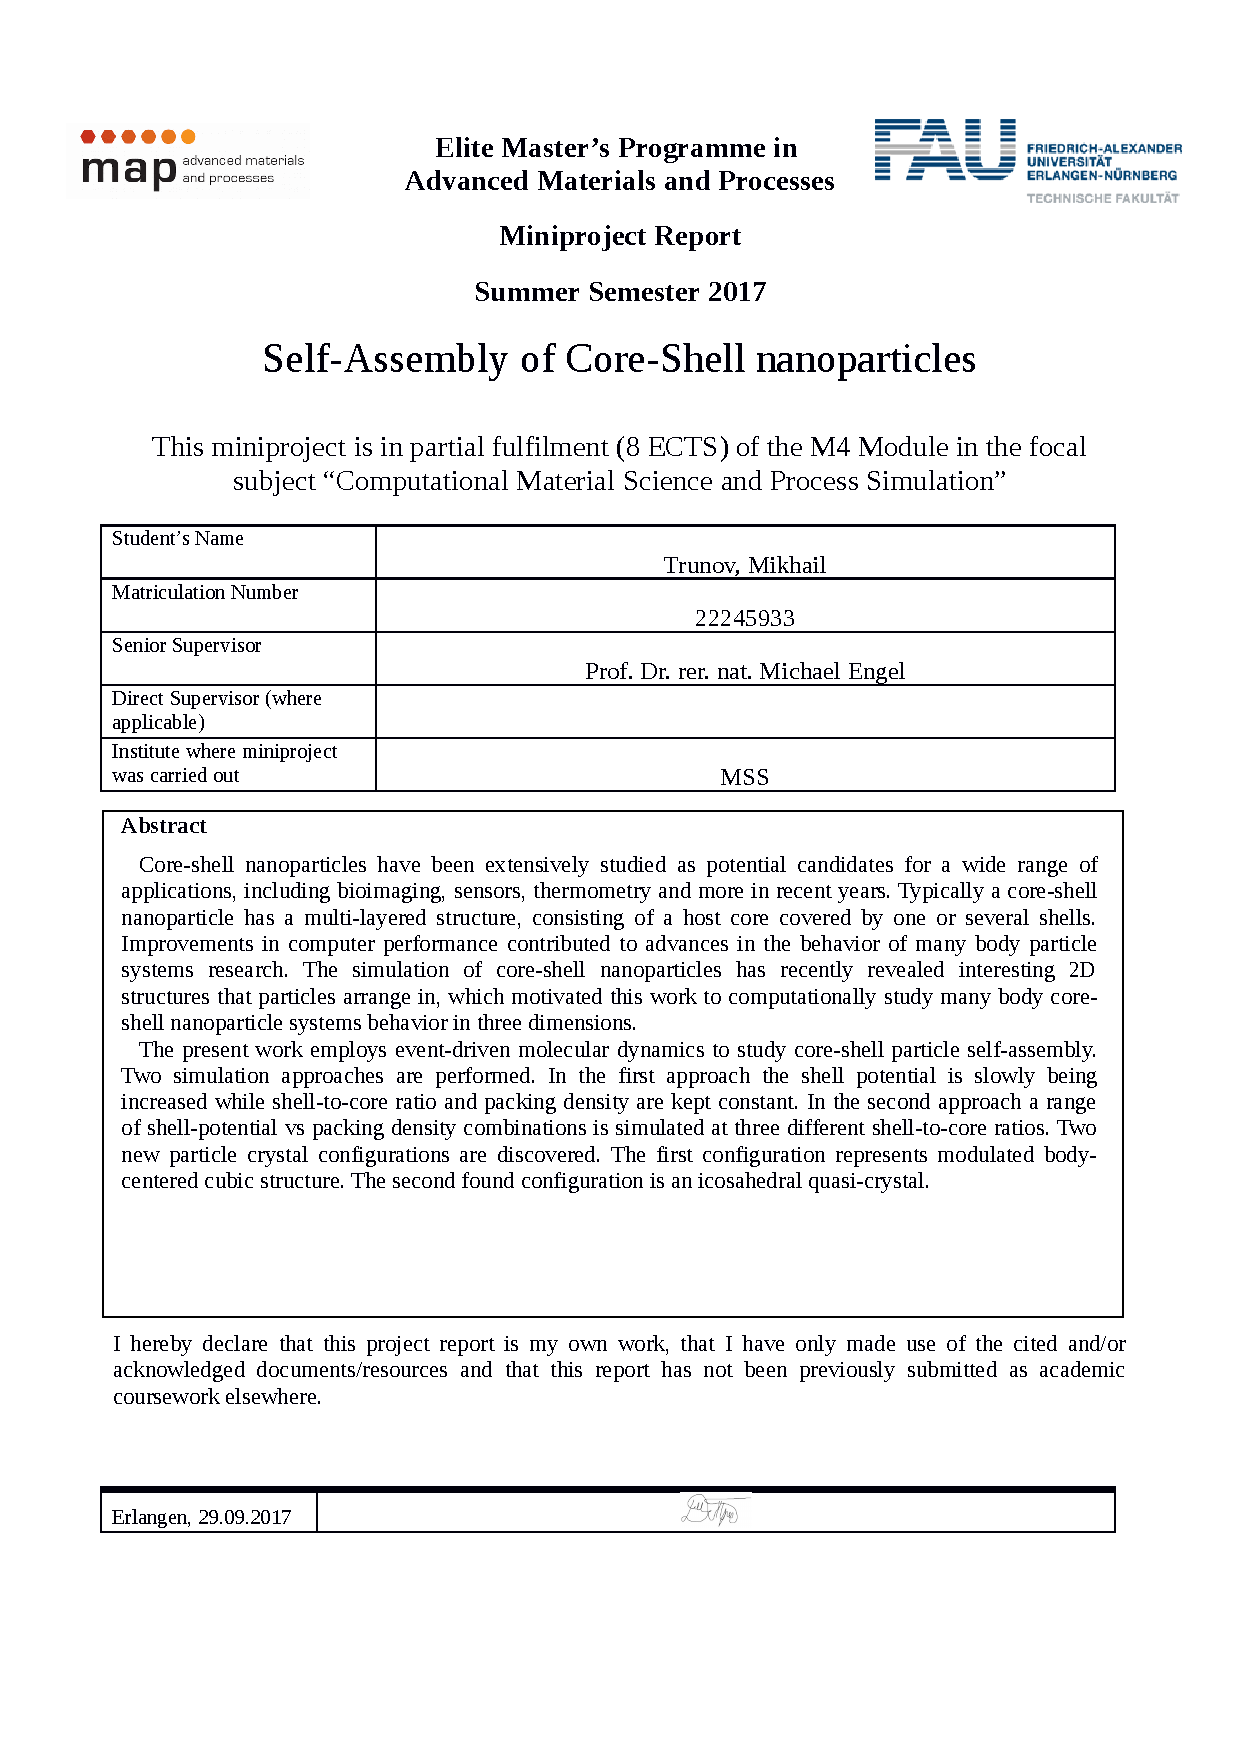
\includepdf[pages={1-2}]{title.pdf}
\section{Introduction}

As pointed out by %Whitesides and Grzybowski
\citet{sadef} the interest in self-assembly (SA) phenomenon is powered by a range of reasons -- from the scientific prospective SA can help understand life and improve the knowledge of the connection between systems and their components, while from the technological view SA appears to be a natural manufacturing approach. The term self-assembly does not have a formal definition,\cite{sadef} however according to the studies of %Halley and Winker
\citet{saterm1} as well as %Herr
\citet{saterm2} SA is the non-dissipative process, involving spontaneous organization of  (usually microscopic) self-assembling units  into complex macroscopic structures, which were not present in the system before. 
Self-assembling units can be represented by nanoparticles,\cite{nanopartunit,nanpartun1} block-copolymers,\cite{blockcpunit} various molecules, including peptides,\cite{molecunit} DNA,\cite{dnaunit,dnaunit1} nanoparticles with DNA ligands\cite{mirkin1996dna} and many more. Self-assembly of nanoparticles can lead to the emergence of materials with unique optical,\cite{opticalex} catalytic\cite{catalitprop} and many other properties. The potential applications of self-assembled materials are biosensors,\cite{optappl} drug delivery\cite{drugappl} and more. A comprehensive review on the self-assembled nanoparticle structures  synthesis, properties and applications was recently published by %Boles et al.
\citet{reviewstart}

The ordered structures of self-assembled nanoparticles can be interesting both from scientific and technological side. First, identifying regular shapes, that nanoparticles arrange in, it is possible to determine the space-fitting units -- basic structures that can fill space, leaving no unoccupied regions, which is referred as tiling. Secondly, the unique structure can define valuable properties. The most intuitive way to tile space is to translate some pattern in non-parallel directions the number of which equals the number of considered space dimensions. The obtained ordered system is referred as periodic crystal structure. However, other ways to tile space with repeating units are possible. If the obtained structures are not periodic but still ordered they are called quasiperiodic. The most know examples of quasiperiodic structures or quasicrystals (QS) are Penrose tilings, which emerged from theoretical investigations. Real-life examples of QCs are usually found in metallic alloys,\cite{qcmetal} while the number of experimental observations of soft matter QCs\cite{qcexper,qctalap} is rather low. In quasiperiodic order space is tiled with a defined set of various shaped units called prototiles. As shown in the review of  %Zhang et al.
\citet{shapes} the synthesis of such prototiles is a possible task, as numerous number of experimentally observed various shaped crystals is reported. In the recent work of %Damasceno et al.
\citet{engelscience} the authors studied space tiling of 145 various polyhedra crystals via Monte Carlo simulations and characterized the observed results into four categories.

An important driving force of nanoparticle self-assembly is entropy, which for some cases is higher for ordered systems, than for disordered ones. Such concept does not seem intuitive, and in fact, as pointed out by %Frenkel
\citet{frenkel2015order} only after 1957 hard sphere spontaneous freezing became a recognized fact due to the experimental evidence and theoretical rationalization.

Self-assembly behavior of nanoparticles is determined by their interaction and surrounding conditions. DLVO theory describes nanoparticle interactions in colloidal systems and considers van der Waals and electrostatic forces between nanoparticles, however %Grasso et al.
\citet{notindlvo} pointed out that for some cases DLVO theory should be significantly extended by other inter-particle forces. The complexity of nanoparticle interactions as well as potential problems of creating particular environment makes it more feasible to study space tiling by nanoparticles via simulations rather than through experimental investigations.

The consideration of all the inter-particle forces is sometimes computationally too expensive, thus idealized models of interacting particles are proposed. The models typically include pair and cluster potentials as well as pair and cluster functionals. The simplest and computationally cheapest model is pair potential. The examples of particle self-assembly simulations  include core-shell,\cite{dotera2014mosaic, coreshell1,stability} Dzugutov,\cite{dzugutpote} Morse\cite{morzepot} and other pair potentials.
%The forces between nanoparticles in colloidal systems are typically described by DLVO theory, however Grasso et al.\cite{notindlvo} pointed out that DLVO theory should be significantly extended by 

Despite simplicity and low number of tunable parameters core-shell potential approximation contributed to the determination of a large number of various structures.\cite{dotera2014mosaic} Particles, possessing core-shell potential behavior can be thought of as nanoparticles with metal or semiconductor hard cores with attached polymer ligands. An example of the experimental research of such system was reported by %Hui et al.
\citet{ligandsexample} 

As shown by several numerical and experimental studies hard bodies like spheres\cite{hardspherepack} or polyhedra\cite{engelscience} can self-assemble into complex structures. The hard-body behavior can be easily obtained varying shell potential strength. Hence, when shell potential is weak, spherical core-shell nanoparticles behave as hard spheres with core radius, while when shell potential is strong, core-shell spherical nanoparticles behave as shell-radius hard objects. %To investigate the hard sphere behavior this study used 

%https://journals.aps.org/prl/abstract/10.1103/PhysRevLett.98.225505#fulltext
%http://iopscience.iop.org/article/10.1088/1367-2630/11/5/053014/meta
%http://pubs.rsc.org/en/content/articlehtml/2014/cc/c4cc06912a

Although the two dimensional core-shell nanoparticle self-assembly is well researched, the formation of three dimensional self-assembled structures is not covered in literature. Hence at present no 3D simulations of core-shell nanoparticles were reported. %Besides, to my knowledge at present no simulations of core-shell particle self-assembled 3D structures for $\lambda=1.4142$ were published.
Thus the present work aims to computationally study self-assembly of core-shell nanoparticles in three dimensions. Two main simulation approaches are used. The first approach is aimed to study the behavior of hard spheres. During the simulations the nanoparticle shell potential is slowly being increased. Experimental representation of such situation can be thought of as slowly increasing the nanoparticle surface coverage by ligands, which can be performed by increasing the ligand concentration in the nanoparticle solution. The purpose of the second simulation approach was to study core-shell nanoparticle behavior in an isolated system. Hence all the parameters, describing particle properties and environment  were kept constant.
%The tiles are divided into periodic and aperiodic. The periodic tiles represent primi
%The uniqueness of self-assembled materials properties can be caused by the order of nanoparticles are structured in space. 

%The main factor, determining properties of  
\section{Simulation and methods}
\subsection{Simulation setup}

The evolution of particle system was investigated via an event-driven molecular dynamics method. Each simulation was run on an ensemble of 2000 core-shell particles in a box with periodic boundary conditions at each boundary. The average kinetic energy of particles was maintained constant using velocity rescaling. Hence, the expression $k_B\cdot T=1$ was maintained through all simulations.
The core-shell pair potential between interacting particles was determined by:
\begin{equation}
U(r)=\begin{cases} 0, r \geq \lambda R_{core} \\ \epsilon, R_{core}<r<\lambda R_{core} \\ \infty, r\leq R_{core} \end{cases},
\end{equation}
here $R_{core}$ -- core radius, $\epsilon$ -- shell potential value, $\lambda$ -- shell to core ratio. 
The packing density value was calculated only considering hard particle cores via:
\begin{equation}
\eta =\frac{4\pi\sum\limits_{i=1}^{2000}R_{core}^3}{3V_{box}},
\end{equation}
where $V_{box}$ denotes the simulation box volume.

The system evolution was analyzed in terms of event-driven molecular dynamics time units. The time unit was considered to be equal to 1. The times between events were calculated using conventional event-driven molecular dynamics approach.\cite{edmd} 

Two simulation approaches were implemented. In the first approach for each simulation the shell to core ratio and packing density were kept constant, while the shell potential was slowly being linearly increased (density vs shell-to-core ratio simulation). The simulation was run for each pair in the ranges 1.15--1.6 and 0.2--0.6 for shell-to-core ratio and packing density respectively. The step in both ranges was 0.05. The step at which shell potential was being increased as well as the maximum and the minimum considered values of shell potential were chosen individually for every packing density and shell-to-core ratio combination. 
At each shell potential value the system was given at least 50 event-driven molecular dynamics time units to equilibrate.  At least 750 event driven molecular dynamics time units were performed in each simulation. 

%Molecular dynamics time was defined in the following way. First 

During another simulation approach all the parameters, including shell potential were kept constant, thus implementing NVT ensemble simulation. Three values of shell-to-core ratio were considered in the current work. For every shell-to-core ratio the simulations were performed in the ranges of 0.5--5 and 0.25--0.55 with incrementing steps of 0.5 and 0.01 for shell potential and packing density respectively. The results were summarized into packing density vs shell-potential phase diagrams for each shell-to-core ratio. %which are given in the section \ref{suppl}. 
The phases on the diagrams are marked with colors. White regions on diagrams mean the phase composition there was not determined and additional simulations are required. Due to limited time each simulation was run once covering at minimum 50 000 event driven molecular dynamics time units. 
%Three shell-to-core ratios were chosen to perform  of  

%The constant temperature of the system was maintained using velocity rescaling.

\subsection{Methods}

The present work employed methods described in the study of \citet{methods} Namely, radial distribution function, diffraction patterns and bond order diagrams were used to investigate the order of self-assembled structures. Due to reasons discussed by \citet{engelscience} here I will not distinguish between FCC and HCP phases.

Radial distribution function (RDF) represents the average particle density at some distance from every particle in the simulation box. It helps to identify long range order in the researched system. %The order is represented by fluctuations

The diffraction patterns of the studied system were obtained by Fourier transform calculations of the particle projections along a chosen axis onto a plane. Each such projection represented a narrow Gaussian distribution. The method simulates electron diffraction experimental material investigations.

The bond orientation order diagrams are the distribution of the bond directions of the closest to a particle neighbors. The distributions are projected onto a sphere surface. 
\section{Results and Discussion}
%\subsection{Event-driven molecular dynamics simulations}
%\subsection{$\eta$ vs $\lambda$ simulations}
\subsection{Density vs shell-to-core ratio simulations}\label{secqc1}

\begin{figure}
 \centering
 \includegraphics[width=0.8\textwidth]{phase1}
\caption{Packing density vs shell-to-core ratio phase diagram. The shell potential is slowly being increased during the simulation} 
\label{fig:phase}
\end{figure}

The simulation with increasing shell potential value revealed the existence of four phases in the studied system (\textbf{Figure} \ref{fig:phase}). As seen from the RDF shapes (\textbf{Figures} \ref{fig:rdf_alpha} and \ref{fig:rdf_beta}) particles in $\alpha$ and $\beta$  phases behave as hard spheres of the shell-size radius. The $\alpha$ phase represents disordered hard-sphere liquid, while the $\beta$ phase has an ordered FCC/HCP %with neighbor distance equal shell radius 
structure, which can be seen from its bond order diagram on the \textbf{Figure} \ref{fig:rdf_beta}. The increase in the value of shell potential for $\alpha$ and $\beta$ phases results in the %initial growth of potential energy of the system, with its subsequent 
potential energy / $\epsilon$ decline to zero (\textbf{Figure} \ref{fig:epot_alpha}), which apparently determines the system equilibrium. 

\begin{figure}%[h]
\centering
\begin{subfigure}{.24\textwidth}
  \centering
  \includegraphics[width=0.98\textwidth]{rdfalpha.tikz}
  \caption{$\alpha$ phase}
  \label{fig:rdf_alpha} 
\end{subfigure}
\begin{subfigure}{.24\textwidth}
  \centering
   \includegraphics[width=0.98\textwidth]{rdfbeta.tikz}
  \caption{$\beta$ phase}
  \label{fig:rdf_beta}  
\end{subfigure}
\begin{subfigure}{.24\textwidth}
  \centering
  \includegraphics[width=0.98\textwidth]{rdfgamma.tikz}
  \caption{$\gamma$ phase}
  \label{fig:rdf_gamma} 
\end{subfigure}
\begin{subfigure}{.24\textwidth}
  \centering
   \includegraphics[width=0.98\textwidth]{rdfdelta.tikz}
  \caption{$\delta$ phase}
  \label{fig:rdf_delta}  
\end{subfigure}
\caption{Typical radial distribution functions and bond order diagrams (for $\beta$ and $\delta$ phases) for simulations with increasing shell potential}
\label{fig:rdf1}
\end{figure}

\begin{figure}
\centering
\begin{subfigure}{.32\textwidth}
  \centering
  \includegraphics[width=0.98\textwidth]{upotalph.tikz}
  \caption{for $\alpha$ and $\beta$ phases}
  \label{fig:epot_alpha} 
\end{subfigure}
\begin{subfigure}{.32\textwidth}
  \centering
   \includegraphics[width=0.98\textwidth]{upotgamm.tikz}
  \caption{for $\gamma$ and $\delta$ phases}
  \label{fig:epot_gamma}  
 \end{subfigure}
% \begin{subfigure}{.24\textwidth}
%   \centering
%    \includegraphics[width=0.98\textwidth]{upot_phi.tikz}
%   \caption{for $\phi$ phase}
%   \label{fig:epot_phi}  
% \end{subfigure}
% \begin{subfigure}{.24\textwidth}
%   \centering
%    \includegraphics[width=0.98\textwidth]{upot_psi.tikz}
%   \caption{for $\psi$ phase}
%   \label{fig:epot_psi}  
% \end{subfigure}
\caption{Typical curves of the potential energy ($E_{pot}$) over shell potential $\epsilon$ evolution vs time for simulations with increasing shell potential}
\label{fig:epot_1}
\end{figure}

High packing density forces particles in $\gamma$ and $\delta$ phases to penetrate into the shells of their neighbors, which is seen in the radial distribution functions behavior (\textbf{Figures} \ref{fig:rdf_gamma} and \ref{fig:rdf_delta}). No order was observed for the $\gamma$ phase region, while particles in the $\delta$ phase were organized into FCC/HCP with neighbor distance equal core radius crystals (\textbf{Figure} \ref{fig:rdf_delta}). The potential energy over shell potential of the system for $\gamma$ and $\delta$ phases  decreased linearly until reaching constant level with the time (\textbf{Figure} \ref{fig:epot_gamma}). %thus repeating the linear growth behavior of the shell potential (\textbf{Figure} \ref{fig:epot_gamma}).

The observed data suggests that particles start to behave as hard bodies and self assemble into close packed structures when packing density reaches the 0.53--0.55 range. The FCC/HCP with neighbor distance equal shell radius structure was observed for packing density 0.53--0.68 considering density was calculated using shell radius. Same tendency to form FCC/HCP with neighbor distance equal core radius structure was observed for $\delta$ phase when the core packing density reached 0.52--0.55 range.

%$\psi$ and $\phi$ phases were only observed for three researched in this study combinations of shell-to-core ratio and shell potential. The phases apparently represent a 5-fold icosahedral QC, which is supported by the bond order diagrams and diffraction patterns shown in the \textbf{Figure} \ref{fig:qc1}. The QC structure was previously reported by Engel et al.\cite{methods} % however the data in this study was too noisy and thus a proper comparison was not performed. 
% The formed structures are different in terms of the particle interactions. Hence in the $\psi$ phase particles probably interact as hard spheres with core radius, while in the $\phi$ phase particle interact as hard spheres with shell radius, which can be derived from radial distribution functions of the phases, shown in the \textbf{Figures} \ref{fig:rdf_phi} and \ref{fig:rdf_psi}. Identical structure of the phases is supported by similar radial distribution function shapes, besides the packing density considering shell radius for $\phi$ phase equals 0.6, while the $\psi$ phase was found at 0.55-0.6 packing density considering core radius.  However, as shown in the \textbf{Figures} \ref{fig:epot_psi} and \ref{fig:epot_phi} the potential energy over the shell potential time evolution behavior does not appear similar for the $\psi$ and $\phi$ phases. The reason is apparently due to the decline in potential energy for $\psi$ phase is comparable with the potential energy fluctuations in the researched system.
%Another QC structure was observed only for one studied in this work shell-to-core ratio vs shell potential combination. The bond order diagram and the diffraction pattern of the phase are shown in the \textbf{Figures} \ref{fig:qcshell} and \ref{fig:dqcshell} 

% \begin{figure}
% \centering
% \begin{subfigure}{.24\textwidth}
%   \centering
%   \includegraphics[width=0.97\textwidth]{rdfS02l145}
%   \caption{}
%   \label{fig:rdf_phi} 
% \end{subfigure}
% \begin{subfigure}{.24\textwidth}
%   \centering
%    \includegraphics[width=0.97\textwidth]{Ds02l145}
%   \caption{}
%   \label{fig:QC_shell_dif}  
% \end{subfigure}
% \begin{subfigure}{.24\textwidth}
%   \centering
%    \includegraphics[width=0.97\textwidth]{rdfS06l13}
%   \caption{}
%   \label{fig:rdf_psi}  
% \end{subfigure}
% \begin{subfigure}{.24\textwidth}
%   \centering
%    \includegraphics[width=0.97\textwidth]{QC_dif1}
%   \caption{}
%   \label{fig:QC_core_dif}  
% \end{subfigure}
% \caption{The radial distribution functions with bond order diagrams and diffraction patterns of the QC structures obtained at $\lambda=1.45$, $\eta=0.2$ (\subref{fig:rdf_phi} and \subref{fig:QC_shell_dif}) and $\lambda=1.3$, $\eta=0.6$ (\subref{fig:rdf_psi} and \subref{fig:QC_core_dif}) for the density vs shell-to-core ratio simulation}
% \label{fig:qc1}
% \end{figure}


%The diffraction pattern together with the bond order diagram of the $\beta$ phase are shown in figure \ref{fig:diff_beta}. As seen from the figure particles are organized into hexagonal close packed (HCP) crystal. Such organization occurs when the potential energy of the system approaches zero. The relation between the potential energy evolution and simulation time of $\beta$ phase has the same pattern as $\alpha$ phase (figure \ref{fig:epot_alpha}). The particles in the formed crystal do not penetrate into each others shells and thus the particles act like spheres with $\lambda$ radius.

%The structure of $\delta$ phase has the order of HCP crystal, however the particles in this phase penetrate into shells and thus form non-zero potential energy structures. Typical radial distribution function is presented in the figure \ref{fig:rdf_delta}. The relation between the potential energy of the phase and $\epsilon$ value has a linear trend. The simulation revealed $\delta$ phase to only form at values of density higher than  0.55 which suggests, that there exists only one particle organization above some critical density point.

%No order was found in the diagram $\gamma$ phase region. Probably, this region has the ability to form complex structures, the size of which significantly exceeds the number of particles, used in simulations of this study.



% \begin{figure}
%     \centering
%     \begin{minipage}{0.47\textwidth}
%         \centering
%         \includegraphics[width=0.97\textwidth]{upotalph.tikz}
% \caption{Typical curve of the potential energy evolution vs simulation time for $\alpha$ and $\beta$ phases}
% \label{fig:epot_alpha}        
%     \end{minipage}\hfill
%     \begin{minipage}{0.47\textwidth}
%         \centering
%  \includegraphics[width=0.97\textwidth]{upotgamm.tikz}
% \caption{Typical curve of the potential energy evolution vs simulation time for $\gamma$ and $\delta$ phases}
% \label{fig:epot_gamma}  
%     \end{minipage}
% \end{figure}



%\subsection{$\epsilon$ vs $\eta$ simulations}
%\clearpage
\subsection{Packing density vs shell potential simulations}

Basing on the previous studies of 2D systems\cite{stability,stability2} it can be concluded that
some interesting structures can self-assemble only in a small range of temperatures and packing densities. Besides, not all shell-to-core ratios contribute to the formation of the rotational order. Taking everything above into account subsequent simulations were performed at constant shell potential and packing density with three shell-to-core ratio values --- $\frac{2}{\sqrt[]{3}}=1.1547$, $\sqrt[]{2}=1.4142$, $\frac{\sqrt{8}}{3}=1.633$. The investigated regions are marked with dashed lines on the \textbf{Figure} \ref{fig:phase}. 

\subsubsection{The 1.1547 shell-to-core ratio}

The value of $\frac{2}{\sqrt[]{3}}=1.1547$ was chosen as it resembles the distance ratio between next-nearest and nearest neighbors in BCC.
The obtained results of the simulation are summarized as phase diagram in the \textbf{Figure} \ref{fig:phase_eta_eps}. As seen from the diagram three phases can be distinguished --- disordered liquid, hard-sphere FCC and BCC. 

\begin{figure}
\centering
\includegraphics[width=0.9\textwidth]{phase1_15_1.tikz}
\caption{Phase diagram packing density $\eta$ vs potential $\epsilon$ at constant $\lambda=1.1547$ with bond order diagrams of the formed phases} \label{fig:phase_eta_epssmall}
\end{figure}

\begin{figure}
\centering
\begin{subfigure}{.61\textwidth}
  \centering
  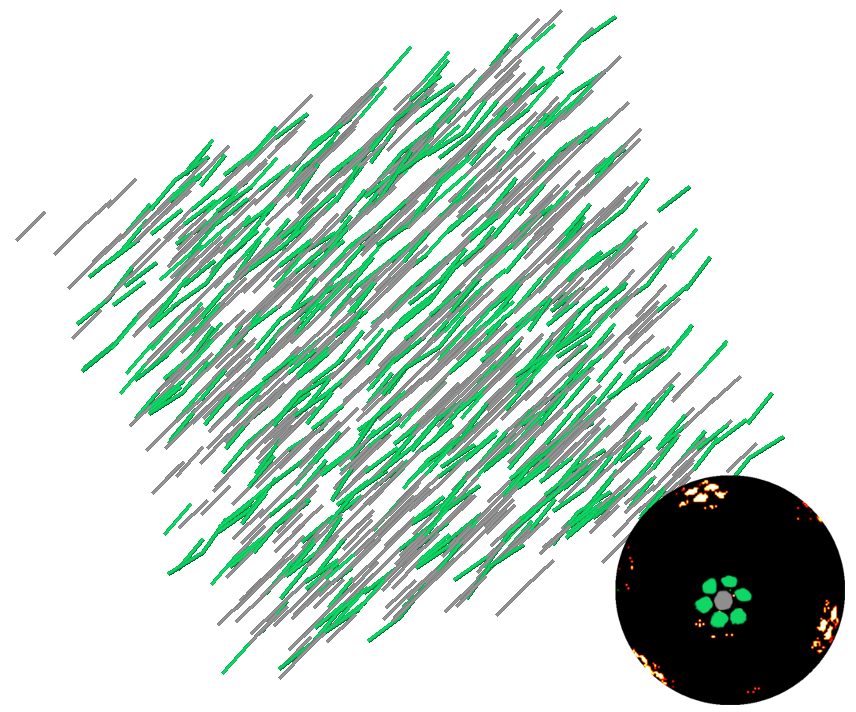
\includegraphics[width=0.98\textwidth]{bonds}
  \caption{}
  \label{fig:bondsmod} 
\end{subfigure}
\begin{subfigure}{.4\textwidth}
  \centering
 \includegraphics[width=0.95\textwidth]{upotmodBCC.tikz}
\caption{}
\label{fig:epot_modBCC} 
\end{subfigure}
\begin{subfigure}{.4\textwidth}
  \includegraphics[width=0.95\textwidth]{rdfmodul.tikz}
\caption{}% of the modulated BCC** phase, obtained at constant  $\lambda=1.1547$ and its deformed unit cell} 
\label{fig:rdfmodul}
\end{subfigure}
\caption{The BCC** structure describing parameters: \subref{fig:bondsmod} -- BCC** bonds distribution, \subref{fig:epot_modBCC} -- typical curve of the evolution of potential energy / $\epsilon$ vs time during the formation of BCC** structure and \subref{fig:rdfmodul} -- typical RDF shape}
\label{fig:modulaphase}
\end{figure}

%     \centering
%     \begin{minipage}{0.31\textwidth}
%         \centering
%         \includegraphics[width=0.95\textwidth]{upotmodBCC.tikz}
% \caption{Typical curve of the evolution of potential energy / $\epsilon$ vs time during the formation of BCC** structure at constant  $\lambda=1.1547$ }
% \label{fig:epot_modBCC}        
%     \end{minipage}\hfill
%     \begin{minipage}{0.45\textwidth}
%         \centering
%  \includegraphics[width=0.95\textwidth]{rdfmodul.tikz}
% \caption{Typical RDF shape of the modulated BCC** phase, obtained at constant  $\lambda=1.1547$ and its deformed unit cell} 
% \label{fig:rdfmodul} 
%     \end{minipage}
% \end{figure}

Modulated BCC** phase was observed at high values of packing density and shell potential.% and thus several simulations with higher than 0.53 packing density were performed. 
The part of the phase diagram where BCC** was observed is shown in the \textbf{Figure} \ref{fig:phase_eta_epssmall}. Here each cross on the phase diagram represents one simulation. The initially formed BCC structure transformed into a more ordered system. The formation of the BCC** phase was observed when the potential energy vs simulation time curve changed the decline shape (\textbf{Figure} \ref{fig:epot_modBCC}). The RDF evolution during BCC to BCC** transition clearly identifies the emergence of higher order among the particle neighbors, lying in 1.5--2.2$R_{core}$ distance range (\textbf{Figure} \ref{fig:rdfmodul}). 
The comparison of bond order diagrams for BCC and BCC** phases suggests that
each BCC bond direction distribution splits in at least seven smaller distributions.



The structure of the obtained BCC** phase has body centered nature, however the BCC unit cells are slightly deformed. The similarly  deformed cells are apparently arranged into some order. The combination of BCC order and the order of equally deformed cells results in the emergence of the observed structure. The \textbf{Figure} \ref{fig:bondsmod} shows the distribution of the bond directions over the crystal. The bond colors  correspond to the color on the bond order diagram. Hence the \textbf{Figure} \ref{fig:bondsmod} demonstrations the existence of some order between gray and green bonds.
%Bond order diagrams of the ordered phases are included in the picture.

\begin{figure}[ht]
\centering
\includegraphics[width=0.67\textwidth]{phase1_15.tikz}
\caption{Phase diagram packing density $\eta$ vs shell potential $\epsilon$ at constant $\lambda=1.1547$} \label{fig:phase_eta_eps}
\end{figure}




% \begin{figure}
% \includegraphics[width=0.9\textwidth]{rdfmodul.tikz}
% \caption{Radial distribution function of the modulated BCC** phase, obtained at constant  $\lambda=1.1547$ } \label{fig:rdfmodul}
% \end{figure}


%\clearpage


\begin{figure}[H]
\centering
\includegraphics[width=0.8\textwidth]{phase1_41.tikz}
\caption{Phase diagram packing density $\eta$ vs shell potential $\epsilon$ at constant $\lambda=1.4142$} \label{fig:phase_1_41}
\end{figure}

\subsubsection{The 1.4142 shell-to-core ratio}

Several studies\cite{dotera2014mosaic,stability} reported the existence of 2D quasi-periodic structures for the shell-to-core ratio of $\sqrt{2}$ %as well as the results from the section \ref{secqc1} where QC was found for close to 1.41 value 
which was a motivation to explore the $\sqrt{2}$ shell-to-core ratio in greater detail for 3D simulations.

Five phases were identified for the considered in the study $\eta-\epsilon$ range for $\lambda=1.4142$ -- disordered liquid, FCC/HCP with neighbor distance equal core radius,  QC, and two transition phases. No ordered structure was observed in the 0.25--0.50 packing density range. Hence the range is not included into the obtained $\eta-\epsilon$ phase diagram which is shown in the \textbf{Figure}  \ref{fig:phase_1_41}. % Another periodic structure was observed at 

\begin{figure}
\centering
%%%%%%%%% RDF
%FCC
\begin{subfigure}{.24\textwidth}
  \centering
  \includegraphics[width=0.97\textwidth]{r141s54e05.tikz}
  %\caption{}
  \label{fig:rdf141fcc} 
\end{subfigure}
% phase 1
\begin{subfigure}{.24\textwidth}
  \centering
  \includegraphics[width=0.97\textwidth]{r141s54e1.tikz}
  %\caption{}
  \label{fig:rdf14phase1} 
\end{subfigure}
% phase 2
\begin{subfigure}{.24\textwidth}
  \centering
  \includegraphics[width=0.97\textwidth]{r141s55e1.tikz}
  %\caption{}
  \label{fig:rdf14phase2} 
\end{subfigure}
% qc
\begin{subfigure}{.24\textwidth}
  \centering
  \includegraphics[width=0.97\textwidth]{r141s53e35.tikz}
  %\caption{}
  \label{fig:rdf14qc} 
\end{subfigure}
%%%%%%%%%%%%BOND
%FCC
\begin{subfigure}{.24\textwidth}
  \centering
   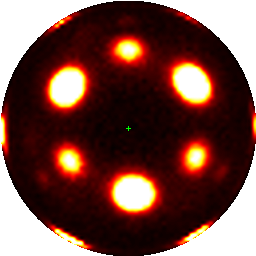
\includegraphics[width=0.67\textwidth]{l141s54e05}
  %\caption{}
  \label{fig:bond141fcc}  
\end{subfigure}
% phase 1
\begin{subfigure}{.24\textwidth}
  \centering
   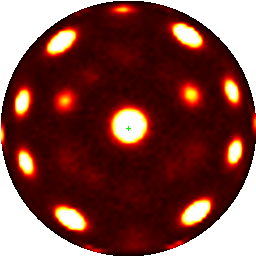
\includegraphics[width=0.67\textwidth]{l141s54e1}
 % \caption{}
  \label{fig:bond141phase1}  
\end{subfigure}
% phase 2
\begin{subfigure}{.24\textwidth}
  \centering
   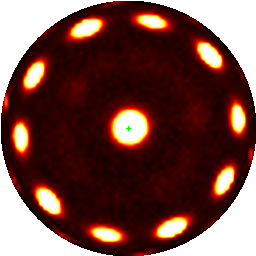
\includegraphics[width=0.67\textwidth]{l141s55e1}
  %\caption{}
  \label{fig:bond141phase2}  
\end{subfigure}
% qc
\begin{subfigure}{.24\textwidth}
  \centering
   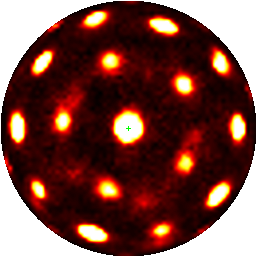
\includegraphics[width=0.67\textwidth]{l141s53e35}
  %\caption{}
  \label{fig:bond141qc}  
\end{subfigure}
%%%%%%%% Difff
%FCC
\begin{subfigure}{.24\textwidth}
  \centering
  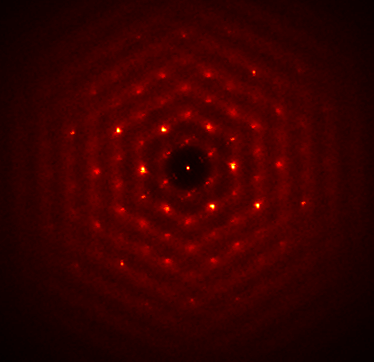
\includegraphics[width=0.95\textwidth]{dl141s54e05}
  \caption{}
  \label{fig:diff141fcc} 
\end{subfigure}
% phase 1
\begin{subfigure}{.24\textwidth}
  \centering
  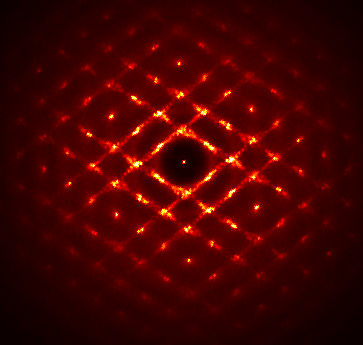
\includegraphics[width=0.95\textwidth]{dl141s54e1}
  \caption{}
  \label{fig:diff141phase1} 
\end{subfigure}
% phase 2
\begin{subfigure}{.24\textwidth}
  \centering
  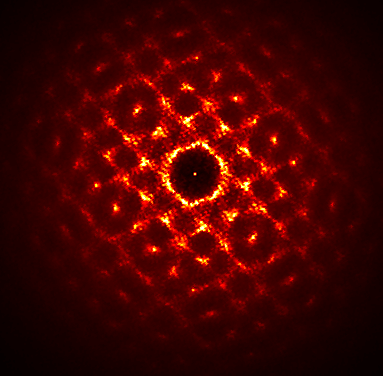
\includegraphics[width=0.95\textwidth]{dl141s55e1}
  \caption{}
  \label{fig:diff141phase2} 
\end{subfigure}
% qc
\begin{subfigure}{.24\textwidth}
  \centering
  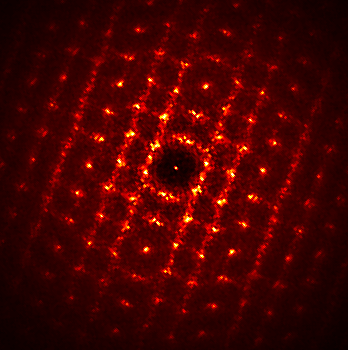
\includegraphics[width=0.95\textwidth]{dl141s53e35}
  \caption{}
  \label{fig:diff141qc} 
\end{subfigure}
\caption{Radial distribution functions, bond order diagrams and diffraction patterns of the structures, formed at  constant $\lambda=1.4142$. \subref{fig:diff141fcc} -- FCC/HCP structure, formed at $\eta=0.54$ and $\epsilon=0.5$, \subref{fig:diff141phase1} -- transition structure, formed at $\eta=0.54$ and $\epsilon=1.0$, \subref{fig:diff141phase2} -- another transition structure, formed at $\eta=0.55$ and $\epsilon=1.0$ and \subref{fig:diff141qc} -- QC structure, formed at $\eta=0.53$ and $\epsilon=3.5$}
\label{fig:evolution141}
\end{figure}

FCC/HCP structure forms at low values of shell potential. The increase in the shell potential forces particles to create transition structures. Two transition structures were recorded during my simulations. The first and the second structures, shown in the \textbf{Figures} \ref{fig:diff141phase1} and  \ref{fig:diff141phase2} respectively have a very similar to FCC/HCP RDF shape. The second structure apparently has a 10-fold symmetry. The formation of the transition structures is accompanied by the reduction of the 3rd peak on FCC/HCP RDF. In the final QC structure the 2nd, 3rd and 4th peaks on RDF have equal height. Basing on the RDFs from the \textbf{Figure} \ref{fig:evolution141} it can be concluded that the QC forms as a result of the particle rearrangement to a closer packed structure, hence the RDF 3rd peak located at about 1.9$R_{core}$ distance reduces its height, which apparently results in the 2nd peak at about 1.5$R_{core}$ distance growth. The moving particles change bond orientations, which is seen from the bond order diagrams. 


%QC structure appears when packing density approaches approximately 0.51. 
Stereographic projections of the bond order diagrams of the obtained QC structure together with the previously reported in the studies of %Engel et al.
\citet{methods} and %Damasceno et al.
\citet{compareicos} icosahedral QSs are shown in the \textbf{Figure} \ref{fig:stereocompare}. 
The shown in the \textbf{Figure} \ref{fig:myqc1} %and \ref{fig:qcfrominc} 
QC structure is similar to the \ref{fig:compare4}, however the RDF and the diffraction pattern appear to be different from previously published results. The QC phase is stable in a large range of varied parameters, however at high shell potential values the QC structure becomes very defective. 
%As seen from the figure the QC has different from the previously published results structure.

\begin{figure}
\centering
\begin{subfigure}{.19\textwidth}
  \centering
  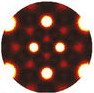
\includegraphics[width=0.97\textwidth]{compare1}
  \caption{}
  \label{fig:compare1} 
\end{subfigure}
\begin{subfigure}{.19\textwidth}
  \centering
   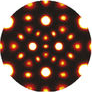
\includegraphics[width=0.97\textwidth]{compare2}
  \caption{}
  \label{fig:compare2}  
\end{subfigure}
%\begin{subfigure}{.19\textwidth}
 % \centering
 % \includegraphics[width=0.97\textwidth]{compare3}
 % \caption{}
 % \label{fig:compare3} 
%\end{subfigure}
\begin{subfigure}{.19\textwidth}
  \centering
  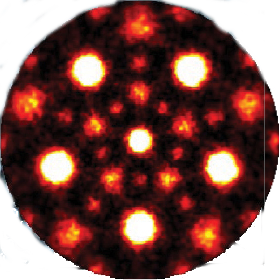
\includegraphics[width=0.97\textwidth]{compare4}
  \caption{}
  \label{fig:compare4} 
\end{subfigure}
\begin{subfigure}{.19\textwidth}
  \centering
   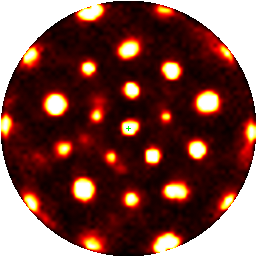
\includegraphics[width=0.97\textwidth]{s_0_53_e_3_50}
  \caption{}
  \label{fig:myqc1}  
\end{subfigure}
%\begin{subfigure}{.19\textwidth}
%  \centering
%   \includegraphics[width=0.97\textwidth]{sincrSters6l13}
%  \caption{}
%  \label{fig:qcfrominc}  
%\end{subfigure}
\caption{Comparison between bond order stereographic projections. Here \subref{fig:compare1}, \subref{fig:compare2} %, \subref{fig:compare3} 
and \subref{fig:compare4} are the projections of icosahedral QCs, obtained in the recent studies,\cite{methods, compareicos} %\subref{fig:myqc} and
\subref{fig:myqc1} %and \subref{fig:qcfrominc} 
--- the QC projection from this work for the parameters %$\lambda=1.4142$, $\eta=0.53$, $\epsilon=0.95$ and 
$\lambda=1.4142$, $\eta=0.53$, $\epsilon=3.5$ %and $\lambda=1.3$, $\eta=0.6$ from section \ref{secqc1} respectively
}
\label{fig:stereocompare}
\end{figure}

%Another observed in this work phase has the %similar to the hard sphere QC (\textbf{Figure} \ref{fig:rdf_psi}) 
%RDF shape, the bond oder diagram as well as the diffraction pattern , shown in the \textbf{Figure} \ref{fig:strangestructure}. 
%The phase probably represents a mixture of several phases.%, one of which is hard sphere .



% \begin{figure}
% \centering
% \begin{subfigure}{.3\textwidth}
%   \centering
%   \includegraphics[width=0.95\textwidth]{rdfstrange.tikz}
%   \caption{}
%   \label{fig:strangerdf} 
% \end{subfigure}
% \begin{subfigure}{.3\textwidth}
%   \centering
%    \includegraphics[width=0.95\textwidth]{s53E95}
%   \caption{}
%   \label{fig:strangebond}  
% \end{subfigure}
% \begin{subfigure}{.3\textwidth}
%   \centering
%   \includegraphics[width=0.95\textwidth]{Diffs53E95}
%   \caption{}
%   \label{fig:strangediff} 
% \end{subfigure}
% \caption{Radial distribution function, bond order diagram and diffraction pattern of the $\beta$ phase obtained at $\eta=0.53$, $\epsilon=1$ and constant $\lambda=1.4142$}
% \label{fig:strangestructure}
% \end{figure}


%The found QC has a unique structure, that does not seem to be previously reported elsewhere. 
%The diffraction patterns and bond order diagrams for various crystal orientations of obtained QC are provided in the \textbf{Figure} \ref{fig:qc2}. %The obtained QC phase seems to be not uniform. 
%Thus for high values of $\epsilon$ quasi-periodic phase is represented %mainly by 5-fold QCs, 
%by two phases while at lower values different quasi-periodic structure is observed. The obtained QC data is less noisy and for high $\epsilon$ values seems to resemble the results from the section \ref{secqc1} and thus a comparison with previously published data is possible. The \textbf{Figure} \ref{fig:stereocompare} shows four  previously observed in the works of Engel et al.\cite{methods} and Damasceno et al.\cite{compareicos} bond order stereographic projections (\textbf{Figures} \ref{fig:compare1}, \ref{fig:compare2}, \ref{fig:compare3} and \ref{fig:compare4}) of icosahedral QCs and %two QC projections 
%one QC projection from this work (\textbf{Figure} % \ref{fig:myqc} and 
%\ref{fig:myqc1}). As seen from the figure the 5-fold QC obtained in this work is different from to my knowledge all the previously published QC structures. The structure on the \textbf{Figure} %\ref{fig:myqc}
%is either same 5-fold QC with defects or another quasi-periodic phase.



% \begin{figure}
% \centering
% \begin{subfigure}{.24\textwidth}
%   \centering
%   \includegraphics[width=0.97\textwidth]{Bond_s_0_53_e_1_50}
%   %\caption{Bond order diagram}
%   \label{fig:qcbond2} 
% \end{subfigure}
% \begin{subfigure}{.24\textwidth}
%   \centering
%    \includegraphics[width=0.97\textwidth]{Diff_s_0_53_e_1_50}
%   %\caption{Diffraction pattern}
%   \label{fig:qcdif2}  
% \end{subfigure}
% \begin{subfigure}{.24\textwidth}
%   \centering
%   \includegraphics[width=0.97\textwidth]{Bond_s_0_53_e_1_50_6}
%   %\caption{Bond order diagram}
%   \label{fig:qcbond2_6} 
% \end{subfigure}
% \begin{subfigure}{.24\textwidth}
%   \centering
%    \includegraphics[width=0.97\textwidth]{Diff_s_0_53_e_1_50_6}
%   %\caption{Diffraction pattern}
%   \label{fig:qcdif2_6}  
% \end{subfigure}
% \caption{The bond order diagrams and diffraction patterns of the QC structure obtained at $\lambda=1.4142$, $\eta=0.53$ and $\epsilon=1.5$ for various crystal orientations}
% \label{fig:qc2}
% \end{figure}




%Thus Dotera et al.\cite{dotera2014mosaic} observed 12-fold QC for 
%The choice of shell-to-core ratio of $\sqrt[]{2}$ was motivated by recent reports of 2D quasi-periodic structures successful findings 
%\clearpage
\subsubsection{The 1.633 shell-to-core ratio}

The ratio of the axes in an ideally dense hexagonal packing equals $\frac{\sqrt{8}}{3}=1.633$, which became the motivation to use this number as a shell-to-core ratio in the simulations.

No ordered phase was observed for all the considered in this work packing density values in the range from 0.25 to 0.52.%, thus the packing density range was expanded up to the value of 0.55. 
The obtained phase diagram is shown in the \textbf{Figure} \ref{fig:phase_1_63}. The disordered phase in the 0.25-0.51 packing density range is not included. 

\begin{figure}
\centering
\includegraphics[width=0.9\textwidth]{phase1_63.tikz}
\caption{Phase diagram packing density $\eta$ vs shell potential $\epsilon$ at constant $\lambda=1.633$} \label{fig:phase_1_63}
\end{figure}

\begin{figure}[H]
% published
\centering
\begin{subfigure}{.24\textwidth}
  \centering
  \includegraphics[width=0.95\textwidth]{brass_published}
  \caption{$\gamma$--Brass}
  \label{fig:brass_p} 
\end{subfigure}
\begin{subfigure}{.24\textwidth}
  \centering
   \includegraphics[width=0.95\textwidth]{b_W_published}
  \caption{$\beta$--W}
  \label{fig:betta_w}  
\end{subfigure}
\begin{subfigure}{.24\textwidth}
  \centering
  \includegraphics[width=0.95\textwidth]{diff_setpf_53_eps_2}
  \caption{$\eta=0.53,\epsilon=2$}
  \label{fig:diff_xz} 
\end{subfigure}
\begin{subfigure}{.24\textwidth}
  \centering
  \includegraphics[width=0.95\textwidth]{diffsetpf_0_54_eps_1_00}
  \caption{$\eta=0.54,\epsilon=1$}
  \label{fig:diff_xz2} 
\end{subfigure}
% Found
\begin{subfigure}{.24\textwidth}
  \centering
  \includegraphics[width=0.95\textwidth]{L_1633_s_0_55_e_2_5}
  \caption{$\eta=0.55,\epsilon=2.5$}
  \label{fig:brass_f} 
\end{subfigure}
\begin{subfigure}{.24\textwidth}
  \centering
   \includegraphics[width=0.95\textwidth]{qc_163_setpf_0_53_eps_1_00}
  \caption{$\eta=0.53,\epsilon=1$}
  \label{fig:betta_w_f}  
\end{subfigure}
\begin{subfigure}{.24\textwidth}
  \centering
  \includegraphics[width=0.95\textwidth]{qc_163_setpf_0_53_eps_2_00}
  \caption{$\eta=0.53,\epsilon=2$}
  \label{fig:bond_xz} 
\end{subfigure}
\begin{subfigure}{.24\textwidth}
  \centering
  \includegraphics[width=0.95\textwidth]{qc_163_setpf_0_54_eps_1_00}
  \caption{$\eta=0.54,\epsilon=1$}
  \label{fig:bond_xz2} 
\end{subfigure}
\caption{Bond order diagrams and diffraction patterns, observed during simulations at constant $\lambda=1.633$. \subref{fig:brass_p} and \subref{fig:betta_w} -- previously reported bond order diagrams, \subref{fig:diff_xz}, \subref{fig:diff_xz2}, \subref{fig:brass_f}, \subref{fig:betta_w_f}, \subref{fig:bond_xz} and \subref{fig:bond_xz2} -- diffraction patterns and bond order diagrams observed in this work.}
\label{fig:allfrom163}
\end{figure}

At the packing density of 0.55 the diagram is mostly occupied by FCC, however %it seems that 
in very small regions the emergence of QC phase is also possible.
Thus at $\epsilon=2.5$, $\eta=0.55$ and  $\epsilon=1$, $\eta=0.53$  $\gamma$-brass and $\beta$--W phases were observed respectively. Previously reported as well as observed in this work bond order diagrams for the $\gamma$-brass and $\beta$--W phases\cite{engelscience} are shown in the \textbf{Figures} \ref{fig:brass_p}, \ref{fig:brass_f}, \ref{fig:betta_w} and \ref{fig:betta_w_f}.

The bond order diagrams as well as the diffraction patterns of the structures, that were not identified by me in the previously published works are shown in the \textbf{Figures} \ref{fig:diff_xz}, \ref{fig:diff_xz2}, \ref{fig:bond_xz} and \ref{fig:bond_xz2}.
%The structure was obtained in the study of Damasceno et al.\cite{engelscience} during truncated dodecahedra simulations. Another complex structure appears in the region with $\epsilon=1-2$ and $\eta=0.53-0.54$. The structure is apparently a 12-fold QC.






\section{Conclusion}

Two new configurations in which core-shell particles arrange in space were discovered in this study. The first configuration was observed for the shell-to-core ratio of 1.1547. The configuration represents a more complex form of a BCC structure. Equally deformed BCC unit cells arrange in an ordered pattern, which is thermodynamically more favorable for the system rather than BCC. The second configuration found in this work is apparently an icosahedral quasi-crystal. The QC was observed for close to $\sqrt[]{2}$ shell-to-core ratios. The evolution of FCC transformation into QC was discussed.

Several crystal configurations were reproduced in this study. %Thus previously reported icosahedral quasi-crystal was observed. %The observed QC appears when packing density of hard spheres reaches 0.6. Other conditions that have to be fulfilled for the QC emergence are to be determined. 
The crystal configurations observed here for shell-to-core ratio of 1.633 were previously found by %Damasceno et al.
\citet{engelscience} However the authors simulated hard polyhedra particles instead of core-shell spherical ones.

The first employed here simulation approach with slowly increasing shell potential value  helped to identify the regions where particles behave as hard spheres either of shell or core radius. Identical packing density values of 0.53-0.55 were observed for the core radius and the shell radius nanoparticles when they started behaving as ordered hard spheres. %both of core and shell radius values .
%of the density vs shell-to-core ratio phase diagram with potential QC structures. However, several phases from constant shell potential simulations were not observed during the density vs shell-to-core ratio simulations, which gives the additional evidence that some phases only occur in regions with limited parameter boundaries. 

The second simulation approach with fixed shell-to-core ratio is better at phase identifications, but the approach is slower as it requires to iterate through the three parameters.

Based on the obtained results there are still several unanswered in this work questions, which can be addressed in the future research. Hence the order of the space positions of deformed BCC unit cells in BCC** phase was not determined. Besides a proper analysis of QC structures obtained at 1.4142 shell-to-core ratio should be performed.  %Do the found structures relate to one QC configuration, or the observed data describes different phases? 
The detailed structure analysis should also be performed for the QCs found at 1.633 shell-to-core ratio. Another potential research direction is the refinement of the discovered here phase boundaries. Hence the transition phases found at $\lambda=1.4142$ simulations seem to occur in a rather small shell potential range. 
The detailed determination of the phase boundaries could be further investigated.
%of are to be determined.

\section*{Acknowledgments}
I would like to thank my supervisor Professor Michael Engel for the support, all the provided to me resources and wonderful experience of participation in the life of his team and the Institute for Multiscale Simulation. I would like to acknowledge Marco Klement for help with technical issues. %This work would be impossible 


% \clearpage

\bibliography{citations}


%\input{supplementary}

\end{document}

%\maketitle

%\thispagestyle{empty}
%\clearpage

%\begin{abstract}
%Core-shell nanoparticles have been extensively studied as potential candidates for a wide range of applications, including bioimaging, sensors, thermometry and more in recent years. Typically a core-shell nanoparticle has a multi-layered structure, consisting of a host core covered by one or several shells. Improvements in computer performance contributed to advances in the behavior of many body particle systems research. The simulation of core-shell nanoparticles has recently revealed interesting 2D structures that particles arrange in, which motivated this work to computationally study many body core-shell nanoparticle systems behavior in three dimensions.

%Self-assembly of core-shell nanoparticles 
%The reasons behind the interest in this material  

%The present work employs event-driven molecular dynamics to study core-shell particle self-assembly. Two simulation approaches are performed. In the first approach the shell potential is slowly being increased while shell-to-core ratio and packing density are kept constant. In the second approach a range of shell-potential vs packing density combinations is simulated at three different shell-to-core ratios. Two new particle crystal configurations are discovered. The first configuration represents modulated body-centered cubic structure. The second found configuration is an icosahedral quasi-crystal. 
%\end{abstract}